\documentclass[11pt,nenglish]{article} % use larger type; default would be 10pt
\newcommand{\XtoCDoku}{1}\newcommand{\XcHomePath}{/media/Data/X2C_v1780}
\usepackage{\XcHomePath/Documentation/General/Styles/generalDoc}
\usepackage{\XcHomePath/Documentation/X2C.VersionInfo}

%\usepackage{todonotes}

\title{Audio\\Library Documentation\\\normalsize X2C v\VersionInfo}
\author{LCM}
\newcommand{\ExtendedBlockDocu}{}
\begin{document}
\selectlanguage{american}
\maketitle
\tableofcontents{}
\newpage

\IfFileExists{../../Library/Audio/Audio.tex}{\section{Audio}
%\XtoCBlock{SineWave}
\label{block:SineWave}
\begin{figure}[H]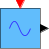
\includegraphics{SineWave}\end{figure} 
%\missingfigure{SineWave : SineWave.png} 

\begin{XtoCtabular}{Outports}
u & Sine wave output\tabularnewline
\hline
\end{XtoCtabular}

\begin{XtoCtabular}{Mask Parameters}
Amplitude & Amplitude of wave\tabularnewline
\hline
Frequency & Frequency in Hz\tabularnewline
\hline
Offset & Offset\tabularnewline
\hline
Phase & Phase [-Pi..Pi]\tabularnewline
\hline
ts\_fact & Multiplication factor of base sampling time (in integer format)\tabularnewline
\hline
\end{XtoCtabular}

\subsubsection*{Description:}
Generation of a sine wave.

% include optional documentation file
\InputIfFileExists{\XcHomePath/Library/Audio/Doc/SineWave_Info.tex}{\vspace{1ex}}{}

\subsubsection*{Implementations:}
\begin{tabular}{l l}
\textbf{FiP8} & 8 Bit Fixed Point Implementation\tabularnewline
\textbf{FiP16} & 16 Bit Fixed Point Implementation\tabularnewline
\textbf{FiP32} & 32 Bit Fixed Point Implementation\tabularnewline
\textbf{Float32} & 32 Bit Floating Point Implementation\tabularnewline
\textbf{Float64} & 64 Bit Floating Point Implementation\tabularnewline
\end{tabular}

\XtoCImplementation{FiP8}
\nopagebreak[0]

8 Bit Fixed Point Implementation

\begin{XtoCtabular}{Outports Data Type}
u & int8\tabularnewline
\hline
\end{XtoCtabular}

\ifdefined \AddTestReports
\InputIfFileExists{\XcHomePath/Library/Audio/Doc/Test-Results/Test_SineWave_FiP8.tex}{}{}
\fi
\XtoCImplementation{FiP16}
\nopagebreak[0]

16 Bit Fixed Point Implementation

\begin{XtoCtabular}{Outports Data Type}
u & int16\tabularnewline
\hline
\end{XtoCtabular}

\ifdefined \AddTestReports
\InputIfFileExists{\XcHomePath/Library/Audio/Doc/Test-Results/Test_SineWave_FiP16.tex}{}{}
\fi
\XtoCImplementation{FiP32}
\nopagebreak[0]

32 Bit Fixed Point Implementation

\begin{XtoCtabular}{Outports Data Type}
u & int32\tabularnewline
\hline
\end{XtoCtabular}

\ifdefined \AddTestReports
\InputIfFileExists{\XcHomePath/Library/Audio/Doc/Test-Results/Test_SineWave_FiP32.tex}{}{}
\fi
\XtoCImplementation{Float32}
\nopagebreak[0]

32 Bit Floating Point Implementation

\begin{XtoCtabular}{Outports Data Type}
u & float32\tabularnewline
\hline
\end{XtoCtabular}

\ifdefined \AddTestReports
\InputIfFileExists{\XcHomePath/Library/Audio/Doc/Test-Results/Test_SineWave_Float32.tex}{}{}
\fi
\XtoCImplementation{Float64}
\nopagebreak[0]

64 Bit Floating Point Implementation

\begin{XtoCtabular}{Outports Data Type}
u & float64\tabularnewline
\hline
\end{XtoCtabular}

\ifdefined \AddTestReports
\InputIfFileExists{\XcHomePath/Library/Audio/Doc/Test-Results/Test_SineWave_Float64.tex}{}{}
\fi

%\XtoCBlock{SineWave}
\label{block:SineWave}
\begin{figure}[H]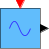
\includegraphics{SineWave}\end{figure} 
%\missingfigure{SineWave : SineWave.png} 

\begin{XtoCtabular}{Outports}
u & Sine wave output\tabularnewline
\hline
\end{XtoCtabular}

\begin{XtoCtabular}{Mask Parameters}
Amplitude & Amplitude of wave\tabularnewline
\hline
Frequency & Frequency in Hz\tabularnewline
\hline
Offset & Offset\tabularnewline
\hline
Phase & Phase [-Pi..Pi]\tabularnewline
\hline
ts\_fact & Multiplication factor of base sampling time (in integer format)\tabularnewline
\hline
\end{XtoCtabular}

\subsubsection*{Description:}
Generation of a sine wave.

% include optional documentation file
\InputIfFileExists{\XcHomePath/Library/Audio/Doc/SineWave_Info.tex}{\vspace{1ex}}{}

\subsubsection*{Implementations:}
\begin{tabular}{l l}
\textbf{FiP8} & 8 Bit Fixed Point Implementation\tabularnewline
\textbf{FiP16} & 16 Bit Fixed Point Implementation\tabularnewline
\textbf{FiP32} & 32 Bit Fixed Point Implementation\tabularnewline
\textbf{Float32} & 32 Bit Floating Point Implementation\tabularnewline
\textbf{Float64} & 64 Bit Floating Point Implementation\tabularnewline
\end{tabular}

\XtoCImplementation{FiP8}
\nopagebreak[0]

8 Bit Fixed Point Implementation

\begin{XtoCtabular}{Outports Data Type}
u & int8\tabularnewline
\hline
\end{XtoCtabular}

\ifdefined \AddTestReports
\InputIfFileExists{\XcHomePath/Library/Audio/Doc/Test-Results/Test_SineWave_FiP8.tex}{}{}
\fi
\XtoCImplementation{FiP16}
\nopagebreak[0]

16 Bit Fixed Point Implementation

\begin{XtoCtabular}{Outports Data Type}
u & int16\tabularnewline
\hline
\end{XtoCtabular}

\ifdefined \AddTestReports
\InputIfFileExists{\XcHomePath/Library/Audio/Doc/Test-Results/Test_SineWave_FiP16.tex}{}{}
\fi
\XtoCImplementation{FiP32}
\nopagebreak[0]

32 Bit Fixed Point Implementation

\begin{XtoCtabular}{Outports Data Type}
u & int32\tabularnewline
\hline
\end{XtoCtabular}

\ifdefined \AddTestReports
\InputIfFileExists{\XcHomePath/Library/Audio/Doc/Test-Results/Test_SineWave_FiP32.tex}{}{}
\fi
\XtoCImplementation{Float32}
\nopagebreak[0]

32 Bit Floating Point Implementation

\begin{XtoCtabular}{Outports Data Type}
u & float32\tabularnewline
\hline
\end{XtoCtabular}

\ifdefined \AddTestReports
\InputIfFileExists{\XcHomePath/Library/Audio/Doc/Test-Results/Test_SineWave_Float32.tex}{}{}
\fi
\XtoCImplementation{Float64}
\nopagebreak[0]

64 Bit Floating Point Implementation

\begin{XtoCtabular}{Outports Data Type}
u & float64\tabularnewline
\hline
\end{XtoCtabular}

\ifdefined \AddTestReports
\InputIfFileExists{\XcHomePath/Library/Audio/Doc/Test-Results/Test_SineWave_Float64.tex}{}{}
\fi

\graphicspath{{Doc/}} \renewcommand{\InputPath}{Doc/} \XtoCBlock{RectangleWave}
\label{block:RectangleWave}
\begin{figure}[H]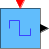
\includegraphics{RectangleWave}\end{figure} 
%\missingfigure{RectangleWave : RectangleWave.png} 

\begin{XtoCtabular}{Outports}
u & Rectangle wave output\tabularnewline
\hline
\end{XtoCtabular}

\begin{XtoCtabular}{Mask Parameters}
Amplitude & Amplitude of wave\tabularnewline
\hline
Frequency & Frequency in Hz\tabularnewline
\hline
Offset & Offset\tabularnewline
\hline
Duty & Duty Cycle in \%\tabularnewline
\hline
ts\_fact & Multiplication factor of base sampling time (in integer format)\tabularnewline
\hline
\end{XtoCtabular}

\subsubsection*{Description:}
Generation of a rectangular wave.

% include optional documentation file
\InputIfFileExists{\XcHomePath/Library/Audio/Doc/RectangleWave_Info.tex}{\vspace{1ex}}{}

\subsubsection*{Implementations:}
\begin{tabular}{l l}
\textbf{FiP8} & 8 Bit Fixed Point Implementation\tabularnewline
\textbf{FiP16} & 16 Bit Fixed Point Implementation\tabularnewline
\textbf{FiP32} & 32 Bit Fixed Point Implementation\tabularnewline
\textbf{Float32} & 32 Bit Floating Point Implementation\tabularnewline
\textbf{Float64} & 64 Bit Floating Point Implementation\tabularnewline
\end{tabular}

\XtoCImplementation{FiP8}
\nopagebreak[0]

8 Bit Fixed Point Implementation

\begin{XtoCtabular}{Outports Data Type}
u & int8\tabularnewline
\hline
\end{XtoCtabular}

\ifdefined \AddTestReports
\InputIfFileExists{\XcHomePath/Library/Audio/Doc/Test-Results/Test_RectangleWave_FiP8.tex}{}{}
\fi
\XtoCImplementation{FiP16}
\nopagebreak[0]

16 Bit Fixed Point Implementation

\begin{XtoCtabular}{Outports Data Type}
u & int16\tabularnewline
\hline
\end{XtoCtabular}

\ifdefined \AddTestReports
\InputIfFileExists{\XcHomePath/Library/Audio/Doc/Test-Results/Test_RectangleWave_FiP16.tex}{}{}
\fi
\XtoCImplementation{FiP32}
\nopagebreak[0]

32 Bit Fixed Point Implementation

\begin{XtoCtabular}{Outports Data Type}
u & int32\tabularnewline
\hline
\end{XtoCtabular}

\ifdefined \AddTestReports
\InputIfFileExists{\XcHomePath/Library/Audio/Doc/Test-Results/Test_RectangleWave_FiP32.tex}{}{}
\fi
\XtoCImplementation{Float32}
\nopagebreak[0]

32 Bit Floating Point Implementation

\begin{XtoCtabular}{Outports Data Type}
u & float32\tabularnewline
\hline
\end{XtoCtabular}

\ifdefined \AddTestReports
\InputIfFileExists{\XcHomePath/Library/Audio/Doc/Test-Results/Test_RectangleWave_Float32.tex}{}{}
\fi
\XtoCImplementation{Float64}
\nopagebreak[0]

64 Bit Floating Point Implementation

\begin{XtoCtabular}{Outports Data Type}
u & float64\tabularnewline
\hline
\end{XtoCtabular}

\ifdefined \AddTestReports
\InputIfFileExists{\XcHomePath/Library/Audio/Doc/Test-Results/Test_RectangleWave_Float64.tex}{}{}
\fi
 \graphicspath{{.}} \renewcommand{\InputPath}{.} 
\clearpage
%\XtoCBlock{TriangleWave}
\label{block:TriangleWave}
\begin{figure}[H]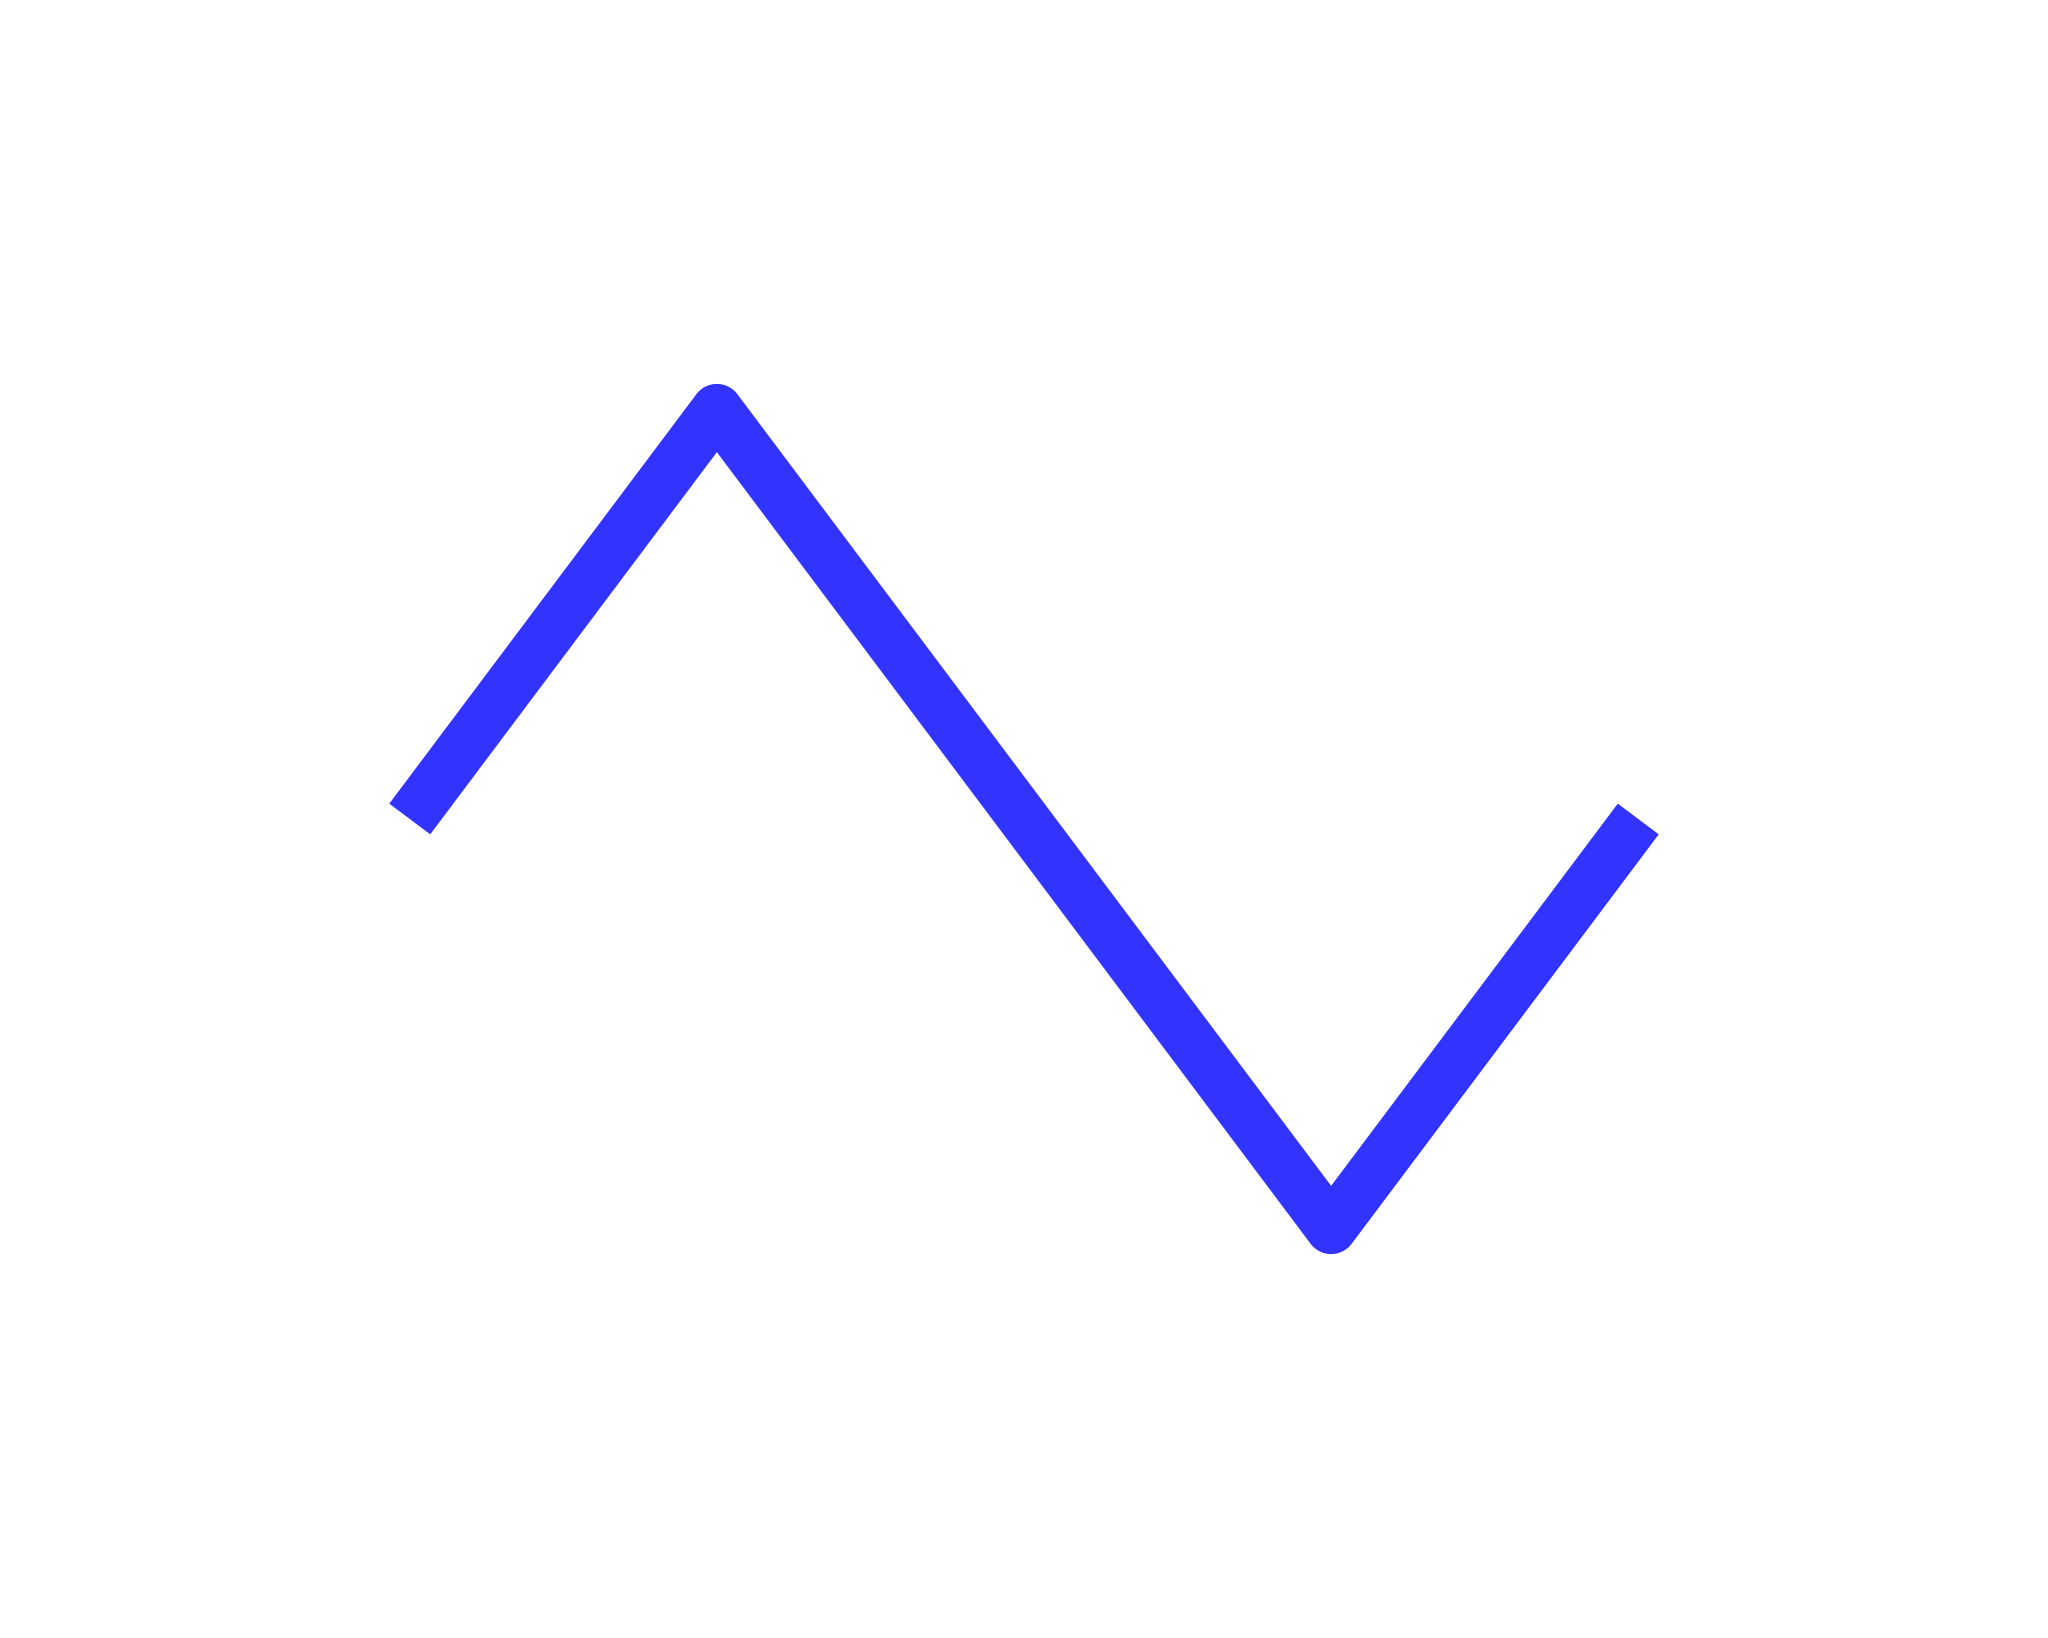
\includegraphics{TriangleWave}\end{figure} 
%\missingfigure{TriangleWave : TriangleWave.png} 

\begin{XtoCtabular}{Outports}
u & Triangle wave output\tabularnewline
\hline
\end{XtoCtabular}

\begin{XtoCtabular}{Mask Parameters}
Amplitude & Amplitude of wave\tabularnewline
\hline
Frequency & Frequency in Hz\tabularnewline
\hline
Offset & Offset\tabularnewline
\hline
Phase & Phase [-Pi..Pi]\tabularnewline
\hline
ts\_fact & Multiplication factor of base sampling time (in integer format)\tabularnewline
\hline
\end{XtoCtabular}

\subsubsection*{Description:}
Generation of a triangular wave.

% include optional documentation file
\InputIfFileExists{\XcHomePath/Library/Audio/Doc/TriangleWave_Info.tex}{\vspace{1ex}}{}

\subsubsection*{Implementations:}
\begin{tabular}{l l}
\textbf{FiP8} & 8 Bit Fixed Point Implementation\tabularnewline
\textbf{FiP16} & 16 Bit Fixed Point Implementation\tabularnewline
\textbf{FiP32} & 32 Bit Fixed Point Implementation\tabularnewline
\textbf{Float32} & 32 Bit Floating Point Implementation\tabularnewline
\textbf{Float64} & 64 Bit Floating Point Implementation\tabularnewline
\end{tabular}

\XtoCImplementation{FiP8}
\nopagebreak[0]

8 Bit Fixed Point Implementation

\begin{XtoCtabular}{Outports Data Type}
u & int8\tabularnewline
\hline
\end{XtoCtabular}

\ifdefined \AddTestReports
\InputIfFileExists{\XcHomePath/Library/Audio/Doc/Test-Results/Test_TriangleWave_FiP8.tex}{}{}
\fi
\XtoCImplementation{FiP16}
\nopagebreak[0]

16 Bit Fixed Point Implementation

\begin{XtoCtabular}{Outports Data Type}
u & int16\tabularnewline
\hline
\end{XtoCtabular}

\ifdefined \AddTestReports
\InputIfFileExists{\XcHomePath/Library/Audio/Doc/Test-Results/Test_TriangleWave_FiP16.tex}{}{}
\fi
\XtoCImplementation{FiP32}
\nopagebreak[0]

32 Bit Fixed Point Implementation

\begin{XtoCtabular}{Outports Data Type}
u & int32\tabularnewline
\hline
\end{XtoCtabular}

\ifdefined \AddTestReports
\InputIfFileExists{\XcHomePath/Library/Audio/Doc/Test-Results/Test_TriangleWave_FiP32.tex}{}{}
\fi
\XtoCImplementation{Float32}
\nopagebreak[0]

32 Bit Floating Point Implementation

\begin{XtoCtabular}{Outports Data Type}
u & float32\tabularnewline
\hline
\end{XtoCtabular}

\ifdefined \AddTestReports
\InputIfFileExists{\XcHomePath/Library/Audio/Doc/Test-Results/Test_TriangleWave_Float32.tex}{}{}
\fi
\XtoCImplementation{Float64}
\nopagebreak[0]

64 Bit Floating Point Implementation

\begin{XtoCtabular}{Outports Data Type}
u & float64\tabularnewline
\hline
\end{XtoCtabular}

\ifdefined \AddTestReports
\InputIfFileExists{\XcHomePath/Library/Audio/Doc/Test-Results/Test_TriangleWave_Float64.tex}{}{}
\fi
 
%\XtoCBlock{TriangleWave}
\label{block:TriangleWave}
\begin{figure}[H]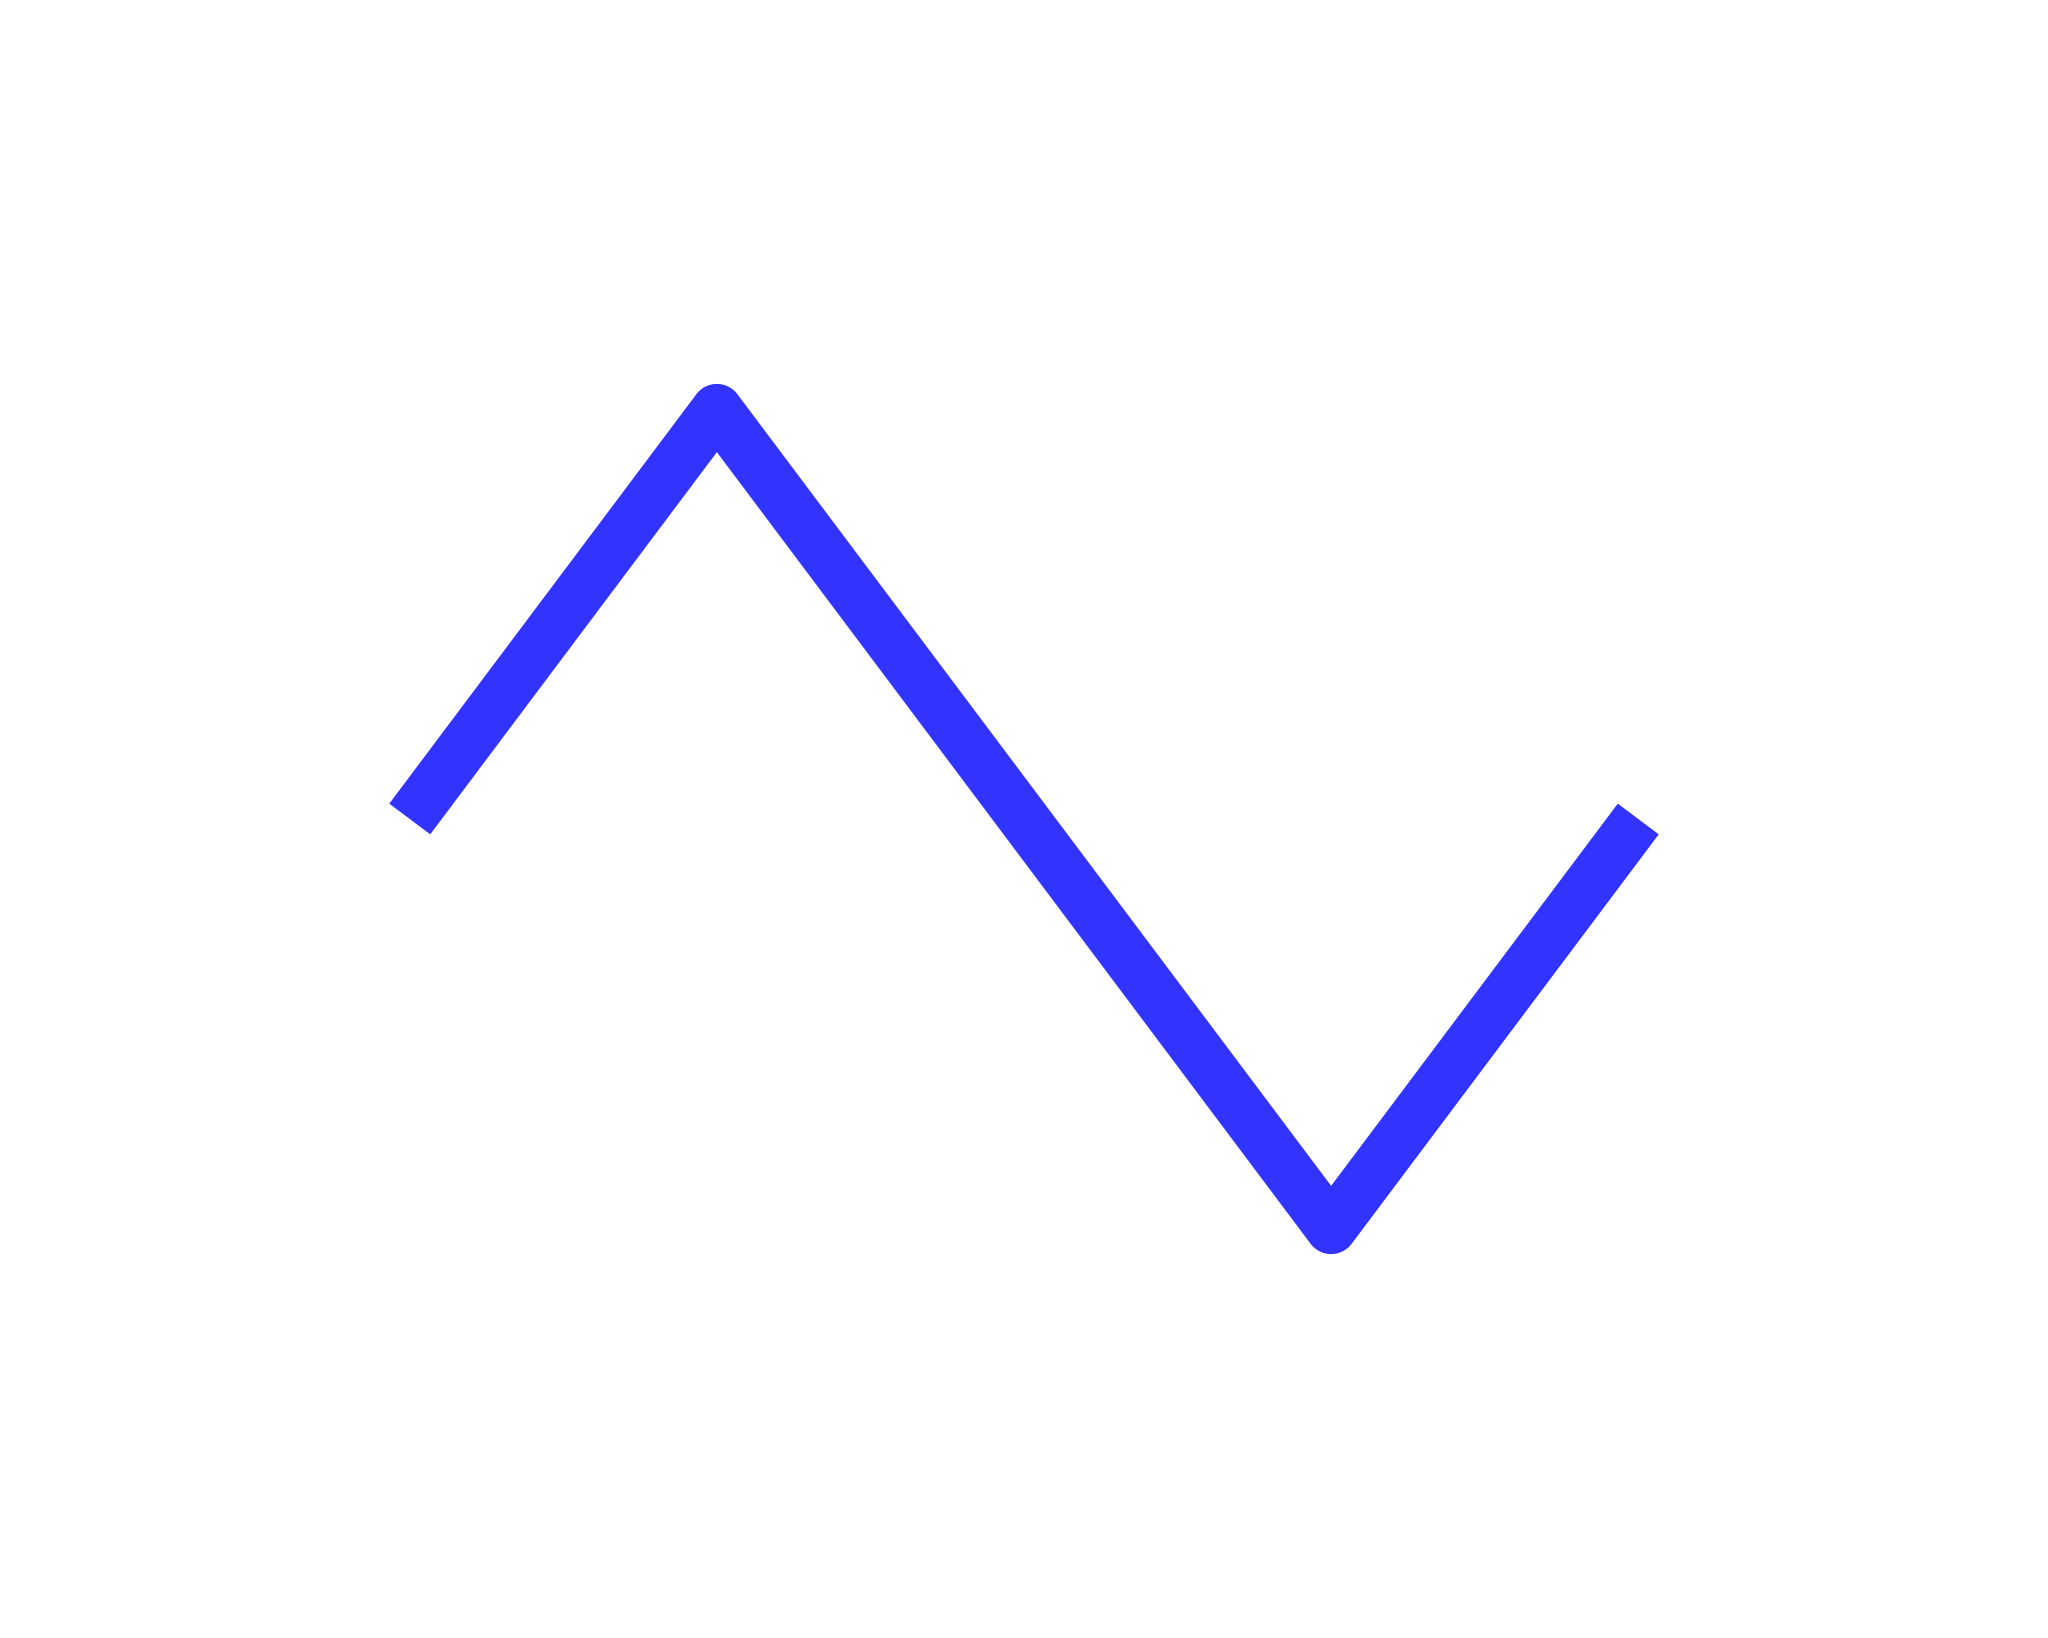
\includegraphics{TriangleWave}\end{figure} 
%\missingfigure{TriangleWave : TriangleWave.png} 

\begin{XtoCtabular}{Outports}
u & Triangle wave output\tabularnewline
\hline
\end{XtoCtabular}

\begin{XtoCtabular}{Mask Parameters}
Amplitude & Amplitude of wave\tabularnewline
\hline
Frequency & Frequency in Hz\tabularnewline
\hline
Offset & Offset\tabularnewline
\hline
Phase & Phase [-Pi..Pi]\tabularnewline
\hline
ts\_fact & Multiplication factor of base sampling time (in integer format)\tabularnewline
\hline
\end{XtoCtabular}

\subsubsection*{Description:}
Generation of a triangular wave.

% include optional documentation file
\InputIfFileExists{\XcHomePath/Library/Audio/Doc/TriangleWave_Info.tex}{\vspace{1ex}}{}

\subsubsection*{Implementations:}
\begin{tabular}{l l}
\textbf{FiP8} & 8 Bit Fixed Point Implementation\tabularnewline
\textbf{FiP16} & 16 Bit Fixed Point Implementation\tabularnewline
\textbf{FiP32} & 32 Bit Fixed Point Implementation\tabularnewline
\textbf{Float32} & 32 Bit Floating Point Implementation\tabularnewline
\textbf{Float64} & 64 Bit Floating Point Implementation\tabularnewline
\end{tabular}

\XtoCImplementation{FiP8}
\nopagebreak[0]

8 Bit Fixed Point Implementation

\begin{XtoCtabular}{Outports Data Type}
u & int8\tabularnewline
\hline
\end{XtoCtabular}

\ifdefined \AddTestReports
\InputIfFileExists{\XcHomePath/Library/Audio/Doc/Test-Results/Test_TriangleWave_FiP8.tex}{}{}
\fi
\XtoCImplementation{FiP16}
\nopagebreak[0]

16 Bit Fixed Point Implementation

\begin{XtoCtabular}{Outports Data Type}
u & int16\tabularnewline
\hline
\end{XtoCtabular}

\ifdefined \AddTestReports
\InputIfFileExists{\XcHomePath/Library/Audio/Doc/Test-Results/Test_TriangleWave_FiP16.tex}{}{}
\fi
\XtoCImplementation{FiP32}
\nopagebreak[0]

32 Bit Fixed Point Implementation

\begin{XtoCtabular}{Outports Data Type}
u & int32\tabularnewline
\hline
\end{XtoCtabular}

\ifdefined \AddTestReports
\InputIfFileExists{\XcHomePath/Library/Audio/Doc/Test-Results/Test_TriangleWave_FiP32.tex}{}{}
\fi
\XtoCImplementation{Float32}
\nopagebreak[0]

32 Bit Floating Point Implementation

\begin{XtoCtabular}{Outports Data Type}
u & float32\tabularnewline
\hline
\end{XtoCtabular}

\ifdefined \AddTestReports
\InputIfFileExists{\XcHomePath/Library/Audio/Doc/Test-Results/Test_TriangleWave_Float32.tex}{}{}
\fi
\XtoCImplementation{Float64}
\nopagebreak[0]

64 Bit Floating Point Implementation

\begin{XtoCtabular}{Outports Data Type}
u & float64\tabularnewline
\hline
\end{XtoCtabular}

\ifdefined \AddTestReports
\InputIfFileExists{\XcHomePath/Library/Audio/Doc/Test-Results/Test_TriangleWave_Float64.tex}{}{}
\fi

\graphicspath{{Doc/}} \renewcommand{\InputPath}{Doc/} \XtoCBlock{SineWave}
\label{block:SineWave}
\begin{figure}[H]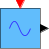
\includegraphics{SineWave}\end{figure} 
%\missingfigure{SineWave : SineWave.png} 

\begin{XtoCtabular}{Outports}
u & Sine wave output\tabularnewline
\hline
\end{XtoCtabular}

\begin{XtoCtabular}{Mask Parameters}
Amplitude & Amplitude of wave\tabularnewline
\hline
Frequency & Frequency in Hz\tabularnewline
\hline
Offset & Offset\tabularnewline
\hline
Phase & Phase [-Pi..Pi]\tabularnewline
\hline
ts\_fact & Multiplication factor of base sampling time (in integer format)\tabularnewline
\hline
\end{XtoCtabular}

\subsubsection*{Description:}
Generation of a sine wave.

% include optional documentation file
\InputIfFileExists{\XcHomePath/Library/Audio/Doc/SineWave_Info.tex}{\vspace{1ex}}{}

\subsubsection*{Implementations:}
\begin{tabular}{l l}
\textbf{FiP8} & 8 Bit Fixed Point Implementation\tabularnewline
\textbf{FiP16} & 16 Bit Fixed Point Implementation\tabularnewline
\textbf{FiP32} & 32 Bit Fixed Point Implementation\tabularnewline
\textbf{Float32} & 32 Bit Floating Point Implementation\tabularnewline
\textbf{Float64} & 64 Bit Floating Point Implementation\tabularnewline
\end{tabular}

\XtoCImplementation{FiP8}
\nopagebreak[0]

8 Bit Fixed Point Implementation

\begin{XtoCtabular}{Outports Data Type}
u & int8\tabularnewline
\hline
\end{XtoCtabular}

\ifdefined \AddTestReports
\InputIfFileExists{\XcHomePath/Library/Audio/Doc/Test-Results/Test_SineWave_FiP8.tex}{}{}
\fi
\XtoCImplementation{FiP16}
\nopagebreak[0]

16 Bit Fixed Point Implementation

\begin{XtoCtabular}{Outports Data Type}
u & int16\tabularnewline
\hline
\end{XtoCtabular}

\ifdefined \AddTestReports
\InputIfFileExists{\XcHomePath/Library/Audio/Doc/Test-Results/Test_SineWave_FiP16.tex}{}{}
\fi
\XtoCImplementation{FiP32}
\nopagebreak[0]

32 Bit Fixed Point Implementation

\begin{XtoCtabular}{Outports Data Type}
u & int32\tabularnewline
\hline
\end{XtoCtabular}

\ifdefined \AddTestReports
\InputIfFileExists{\XcHomePath/Library/Audio/Doc/Test-Results/Test_SineWave_FiP32.tex}{}{}
\fi
\XtoCImplementation{Float32}
\nopagebreak[0]

32 Bit Floating Point Implementation

\begin{XtoCtabular}{Outports Data Type}
u & float32\tabularnewline
\hline
\end{XtoCtabular}

\ifdefined \AddTestReports
\InputIfFileExists{\XcHomePath/Library/Audio/Doc/Test-Results/Test_SineWave_Float32.tex}{}{}
\fi
\XtoCImplementation{Float64}
\nopagebreak[0]

64 Bit Floating Point Implementation

\begin{XtoCtabular}{Outports Data Type}
u & float64\tabularnewline
\hline
\end{XtoCtabular}

\ifdefined \AddTestReports
\InputIfFileExists{\XcHomePath/Library/Audio/Doc/Test-Results/Test_SineWave_Float64.tex}{}{}
\fi
 \graphicspath{{.}} \renewcommand{\InputPath}{.} 
\clearpage
%\XtoCBlock{RectangleWave}
\label{block:RectangleWave}
\begin{figure}[H]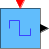
\includegraphics{RectangleWave}\end{figure} 
%\missingfigure{RectangleWave : RectangleWave.png} 

\begin{XtoCtabular}{Outports}
u & Rectangle wave output\tabularnewline
\hline
\end{XtoCtabular}

\begin{XtoCtabular}{Mask Parameters}
Amplitude & Amplitude of wave\tabularnewline
\hline
Frequency & Frequency in Hz\tabularnewline
\hline
Offset & Offset\tabularnewline
\hline
Duty & Duty Cycle in \%\tabularnewline
\hline
ts\_fact & Multiplication factor of base sampling time (in integer format)\tabularnewline
\hline
\end{XtoCtabular}

\subsubsection*{Description:}
Generation of a rectangular wave.

% include optional documentation file
\InputIfFileExists{\XcHomePath/Library/Audio/Doc/RectangleWave_Info.tex}{\vspace{1ex}}{}

\subsubsection*{Implementations:}
\begin{tabular}{l l}
\textbf{FiP8} & 8 Bit Fixed Point Implementation\tabularnewline
\textbf{FiP16} & 16 Bit Fixed Point Implementation\tabularnewline
\textbf{FiP32} & 32 Bit Fixed Point Implementation\tabularnewline
\textbf{Float32} & 32 Bit Floating Point Implementation\tabularnewline
\textbf{Float64} & 64 Bit Floating Point Implementation\tabularnewline
\end{tabular}

\XtoCImplementation{FiP8}
\nopagebreak[0]

8 Bit Fixed Point Implementation

\begin{XtoCtabular}{Outports Data Type}
u & int8\tabularnewline
\hline
\end{XtoCtabular}

\ifdefined \AddTestReports
\InputIfFileExists{\XcHomePath/Library/Audio/Doc/Test-Results/Test_RectangleWave_FiP8.tex}{}{}
\fi
\XtoCImplementation{FiP16}
\nopagebreak[0]

16 Bit Fixed Point Implementation

\begin{XtoCtabular}{Outports Data Type}
u & int16\tabularnewline
\hline
\end{XtoCtabular}

\ifdefined \AddTestReports
\InputIfFileExists{\XcHomePath/Library/Audio/Doc/Test-Results/Test_RectangleWave_FiP16.tex}{}{}
\fi
\XtoCImplementation{FiP32}
\nopagebreak[0]

32 Bit Fixed Point Implementation

\begin{XtoCtabular}{Outports Data Type}
u & int32\tabularnewline
\hline
\end{XtoCtabular}

\ifdefined \AddTestReports
\InputIfFileExists{\XcHomePath/Library/Audio/Doc/Test-Results/Test_RectangleWave_FiP32.tex}{}{}
\fi
\XtoCImplementation{Float32}
\nopagebreak[0]

32 Bit Floating Point Implementation

\begin{XtoCtabular}{Outports Data Type}
u & float32\tabularnewline
\hline
\end{XtoCtabular}

\ifdefined \AddTestReports
\InputIfFileExists{\XcHomePath/Library/Audio/Doc/Test-Results/Test_RectangleWave_Float32.tex}{}{}
\fi
\XtoCImplementation{Float64}
\nopagebreak[0]

64 Bit Floating Point Implementation

\begin{XtoCtabular}{Outports Data Type}
u & float64\tabularnewline
\hline
\end{XtoCtabular}

\ifdefined \AddTestReports
\InputIfFileExists{\XcHomePath/Library/Audio/Doc/Test-Results/Test_RectangleWave_Float64.tex}{}{}
\fi

%\XtoCBlock{RectangleWave}
\label{block:RectangleWave}
\begin{figure}[H]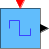
\includegraphics{RectangleWave}\end{figure} 
%\missingfigure{RectangleWave : RectangleWave.png} 

\begin{XtoCtabular}{Outports}
u & Rectangle wave output\tabularnewline
\hline
\end{XtoCtabular}

\begin{XtoCtabular}{Mask Parameters}
Amplitude & Amplitude of wave\tabularnewline
\hline
Frequency & Frequency in Hz\tabularnewline
\hline
Offset & Offset\tabularnewline
\hline
Duty & Duty Cycle in \%\tabularnewline
\hline
ts\_fact & Multiplication factor of base sampling time (in integer format)\tabularnewline
\hline
\end{XtoCtabular}

\subsubsection*{Description:}
Generation of a rectangular wave.

% include optional documentation file
\InputIfFileExists{\XcHomePath/Library/Audio/Doc/RectangleWave_Info.tex}{\vspace{1ex}}{}

\subsubsection*{Implementations:}
\begin{tabular}{l l}
\textbf{FiP8} & 8 Bit Fixed Point Implementation\tabularnewline
\textbf{FiP16} & 16 Bit Fixed Point Implementation\tabularnewline
\textbf{FiP32} & 32 Bit Fixed Point Implementation\tabularnewline
\textbf{Float32} & 32 Bit Floating Point Implementation\tabularnewline
\textbf{Float64} & 64 Bit Floating Point Implementation\tabularnewline
\end{tabular}

\XtoCImplementation{FiP8}
\nopagebreak[0]

8 Bit Fixed Point Implementation

\begin{XtoCtabular}{Outports Data Type}
u & int8\tabularnewline
\hline
\end{XtoCtabular}

\ifdefined \AddTestReports
\InputIfFileExists{\XcHomePath/Library/Audio/Doc/Test-Results/Test_RectangleWave_FiP8.tex}{}{}
\fi
\XtoCImplementation{FiP16}
\nopagebreak[0]

16 Bit Fixed Point Implementation

\begin{XtoCtabular}{Outports Data Type}
u & int16\tabularnewline
\hline
\end{XtoCtabular}

\ifdefined \AddTestReports
\InputIfFileExists{\XcHomePath/Library/Audio/Doc/Test-Results/Test_RectangleWave_FiP16.tex}{}{}
\fi
\XtoCImplementation{FiP32}
\nopagebreak[0]

32 Bit Fixed Point Implementation

\begin{XtoCtabular}{Outports Data Type}
u & int32\tabularnewline
\hline
\end{XtoCtabular}

\ifdefined \AddTestReports
\InputIfFileExists{\XcHomePath/Library/Audio/Doc/Test-Results/Test_RectangleWave_FiP32.tex}{}{}
\fi
\XtoCImplementation{Float32}
\nopagebreak[0]

32 Bit Floating Point Implementation

\begin{XtoCtabular}{Outports Data Type}
u & float32\tabularnewline
\hline
\end{XtoCtabular}

\ifdefined \AddTestReports
\InputIfFileExists{\XcHomePath/Library/Audio/Doc/Test-Results/Test_RectangleWave_Float32.tex}{}{}
\fi
\XtoCImplementation{Float64}
\nopagebreak[0]

64 Bit Floating Point Implementation

\begin{XtoCtabular}{Outports Data Type}
u & float64\tabularnewline
\hline
\end{XtoCtabular}

\ifdefined \AddTestReports
\InputIfFileExists{\XcHomePath/Library/Audio/Doc/Test-Results/Test_RectangleWave_Float64.tex}{}{}
\fi

\graphicspath{{Doc/}} \renewcommand{\InputPath}{Doc/} \XtoCBlock{TriangleWave}
\label{block:TriangleWave}
\begin{figure}[H]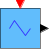
\includegraphics{TriangleWave}\end{figure} 
%\missingfigure{TriangleWave : TriangleWave.png} 

\begin{XtoCtabular}{Outports}
u & Triangle wave output\tabularnewline
\hline
\end{XtoCtabular}

\begin{XtoCtabular}{Mask Parameters}
Amplitude & Amplitude of wave\tabularnewline
\hline
Frequency & Frequency in Hz\tabularnewline
\hline
Offset & Offset\tabularnewline
\hline
Phase & Phase [-Pi..Pi]\tabularnewline
\hline
ts\_fact & Multiplication factor of base sampling time (in integer format)\tabularnewline
\hline
\end{XtoCtabular}

\subsubsection*{Description:}
Generation of a triangular wave.

% include optional documentation file
\InputIfFileExists{\XcHomePath/Library/Audio/Doc/TriangleWave_Info.tex}{\vspace{1ex}}{}

\subsubsection*{Implementations:}
\begin{tabular}{l l}
\textbf{FiP8} & 8 Bit Fixed Point Implementation\tabularnewline
\textbf{FiP16} & 16 Bit Fixed Point Implementation\tabularnewline
\textbf{FiP32} & 32 Bit Fixed Point Implementation\tabularnewline
\textbf{Float32} & 32 Bit Floating Point Implementation\tabularnewline
\textbf{Float64} & 64 Bit Floating Point Implementation\tabularnewline
\end{tabular}

\XtoCImplementation{FiP8}
\nopagebreak[0]

8 Bit Fixed Point Implementation

\begin{XtoCtabular}{Outports Data Type}
u & int8\tabularnewline
\hline
\end{XtoCtabular}

\ifdefined \AddTestReports
\InputIfFileExists{\XcHomePath/Library/Audio/Doc/Test-Results/Test_TriangleWave_FiP8.tex}{}{}
\fi
\XtoCImplementation{FiP16}
\nopagebreak[0]

16 Bit Fixed Point Implementation

\begin{XtoCtabular}{Outports Data Type}
u & int16\tabularnewline
\hline
\end{XtoCtabular}

\ifdefined \AddTestReports
\InputIfFileExists{\XcHomePath/Library/Audio/Doc/Test-Results/Test_TriangleWave_FiP16.tex}{}{}
\fi
\XtoCImplementation{FiP32}
\nopagebreak[0]

32 Bit Fixed Point Implementation

\begin{XtoCtabular}{Outports Data Type}
u & int32\tabularnewline
\hline
\end{XtoCtabular}

\ifdefined \AddTestReports
\InputIfFileExists{\XcHomePath/Library/Audio/Doc/Test-Results/Test_TriangleWave_FiP32.tex}{}{}
\fi
\XtoCImplementation{Float32}
\nopagebreak[0]

32 Bit Floating Point Implementation

\begin{XtoCtabular}{Outports Data Type}
u & float32\tabularnewline
\hline
\end{XtoCtabular}

\ifdefined \AddTestReports
\InputIfFileExists{\XcHomePath/Library/Audio/Doc/Test-Results/Test_TriangleWave_Float32.tex}{}{}
\fi
\XtoCImplementation{Float64}
\nopagebreak[0]

64 Bit Floating Point Implementation

\begin{XtoCtabular}{Outports Data Type}
u & float64\tabularnewline
\hline
\end{XtoCtabular}

\ifdefined \AddTestReports
\InputIfFileExists{\XcHomePath/Library/Audio/Doc/Test-Results/Test_TriangleWave_Float64.tex}{}{}
\fi
 \graphicspath{{.}} \renewcommand{\InputPath}{.} 
\clearpage
}{}\end{document}
\end
